\chapter{Design}

\section{Methodology}

\begin{figure}[!h]
    \caption{Tree-Shape}
    \centering
    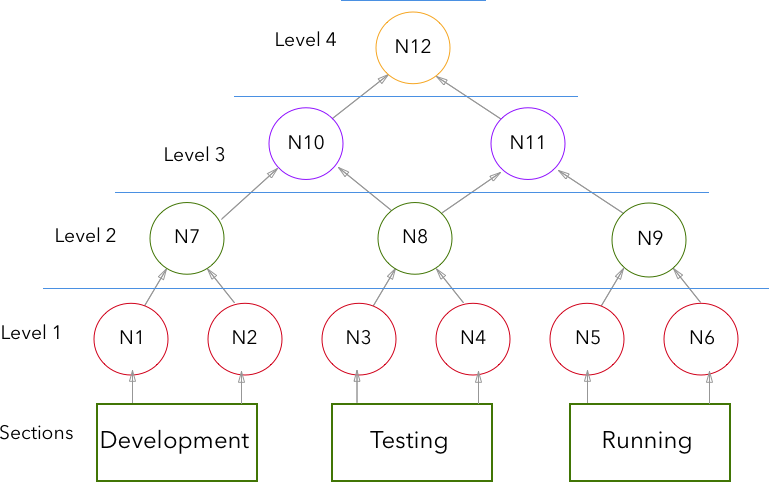
\includegraphics[width=100mm]{images/methodology}
    \label{fig:label}
\end{figure}

% \begin{figure}[!h]
%     \centering
%     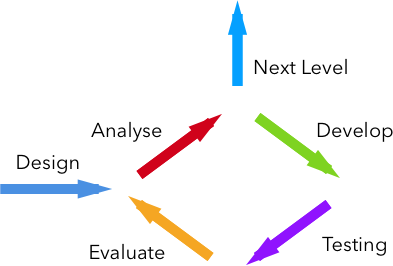
\includegraphics[width=50mm]{images/spiral_model}
%     \label{fig:label}
% \end{figure}

% \begin{figure}[!h]
%     \centering
%     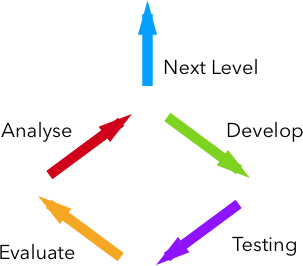
\includegraphics[width=50mm]{images/spiral_model_2}
%     \label{fig:label}
% \end{figure}

After doing research, I decided to implement my methodology called ”Tree-Shaped”. The idea behind this method is to en-corporate the functionality into different sections and prove each functionality at a lower, early stage. This benefits by setting out the goal into sections and filling in what functional requirements are needed to reach the target. The proving of functionality part is to able to fix any potential compatibilities at an earlier stage or remove if necessary.

The methodology has three parts

\begin{enumerate}
  \item Sections
  
    The sections stage is the first step in using this ”tree-shaped”. This part is where we set out what we are trying to achieve. Then incorporate each functionality into their respective sections.
    
  \item Functionality   
    
    After we define our sections including their respective functionalities, tests are to be written out for each functionality. The test shows that they still output the correct result, being what they are supposed to do.
    
  \item Levels
  
   Levels stage is where we are proving/testing the functionalists. As we move up the tree into each node, the functionalists are combined. Thus solving compatibilities issues at an earlier stage of the project development.
\end{enumerate}

\subsection{Advantages}

This methodology based on the test-driven development (TDD) process that relies on the repetition of very short development cycles. At each level, the nodes which hold the application are tested. These tests are from the functionality part when combining the previous nodes to make sure they still output the correct result.

\subsection{Disadvantages}

The methodology although sounds good from a theoretical point of view, but in a real world it has its drawbacks. Each node (circle in each level) requires making new test application, combine the previous two node applications and possible refactoring. This takes time what some projects do not have, but it reduces the number of bugs found by refactoring at each level. To overcome this, the methodology allows skipping one level to reduce testing times.

\section{Functional Requirements}

Functional requirement defines a function of a system or its component. After having discussions with outsourced developers and researching current systems, the following \ref{tb:functional} illustrates the list of functional requirement. They are grouped into sections and what the aim of the project will deliver.

\begin{table}[!h]
\centering
\caption{Functional Requirements}
\label{tb:functional}
\begin{tabular}{|l|l|l|l|l|}
\hline
\cellcolor{green!20}ID & \cellcolor{green!20}Section  & \cellcolor{green!20}Name  & \cellcolor{green!20}Description        & \cellcolor{green!20}Priority \\ \hline
1                      & Development                  & Cloud Storage            & Create, Read, Update, Delete objects   & High   \\ \hline
2                      & Development                  & Push notifications        & Send push notifications to devices     & Medium \\ \hline
3                      & Production                   & Analytics                 & Measure users in app activities        & High   \\ \hline
4                      & Production                   & Backup                    & Backup database to remote site         & Low    \\ \hline
5                      & Development                  & Self hosted               & Host the MBaaS on developers server    & High   \\ \hline
6                      & Production                   & Remote Configuration      & In app live updates                    & High   \\ \hline
7                      & Production                   & A/B Testing               & Testing different variations           & High   \\ \hline
8                      & Development                  & Live Database             & Update objects without user refreshing & Low    \\ \hline
9                      & Development                  & Dashboard                & Interface for developers manage apps   & High   \\ \hline
10                     & Testing                      & Exceptions                 & Tools to collect and view exceptions   & High   \\ \hline
11                     & Testing                      & Test environment      & Testing bugs/issues in a test enviornment & Medium \\ \hline
\end{tabular}
\end{table}

\subsection{Development}

\subsubsection{Cloud Storage} \label{d-d:cloud_storage}

Cloud storage is a service model in which data is managed remotely and made available to users over the Internet. This service allows developers to keep the application data in one or more locations, for the end users to access. Mobile app users want the ability to be connected to others, to share information but without filling up local storage. This cloud service solves this problem by storing the data remotely, and the application makes requests through some protocol to access the user's data. The service will provide tools for the developer to create, read, update and delete the data.

\subsubsection{Sprint board} \label{d-d:sprint_board}
Challenges faced when developing an application, is trying to keep a list of features implemented in each version. There are already different sprint board applications out there, but wanted a way to en-corporate it all in one single dashboard application. This feature will be incorporated with exceptions discussed in section \ref{testing subsection}, where an exception can be attached to a ticket. This will help with tracking issues and signed off once completed.

\subsubsection{Self hosted} \label{d-d:self_hosted}
This will allow the developer to host their system, to have full control of when running, and not to have to worry if the provider is going to shut down the service. By giving the developer a way to host their back-end then this will keep the cost down of not having to pay for third party services.

\subsection{Testing} 

\subsubsection{Exceptions} \label{testing subsection}

When an application crash, the reason for this is called an uncaught exception. An exception is an event, which occurs when the application is running, that disrupts the flow of a set of actions. An exception can occur when trying to read a value from a variable that does not exist. When developing applications, a good design is to handle all potential exceptions. This is known as a caught exception, and the application does not crash. These exceptions can only be seen by the developer when testing the application, but can not always find these potential issues. This project will design a way, which the both uncaught and caught exceptions can send to the developer.

\subsubsection{Test environment} \label{d-t:test_enviornment}

In the exceptions section \ref{testing subsection},we discussed that bugs/issues could occur will application, but testing the application on live data is the wrong approach. This can be done when the application is being tested; a test database will be used without the hassle of creating one. The cloud services currently do not provide a testing environment, where the integrity of the data is a priority. The project will be designed so that when the application is in debug mode, it will use the testing environment.

\subsection{Production}

\subsubsection{Backup} \label{d-p:backup}

During the research when asking developers what services are missing from current mobile cloud services, one was a backup feature. They wanted a way to completely backup their data being files and database contents. This would enable them to both have the piece of mind that their user's data is safe, and to have the option to change cloud service providers. It seems that providers create their systems in such a way that once the developer starts using it, they would not be able to migrate. This is down to not providing a service to transfer their user's data. This system will provide two services: one to backup their data to a remote or local location, and secondly to import data to aid in migrating to using this system.

\subsubsection{A/B Testing} \label{design:abtesting}
A/B testing also known as split testing is comparing two variations of a page to see which performs better. Currently this popular with web pages but my plan is to bring this to mobile applications. All mobile applications no matter what services they provide all have one goal: a reason to exist. A/B testing allows you to make more out of your existing traffic. This is achieved by sending our two variants ( A and B ) to similar visitors at the same time and use analytics to provide display what variation wins. Included in the research, a survey was conducted in section \ref{research:mobile_users} to see what users felt about mobile apps. The results were that end-users do choose whether or not they will continue to use an app based on the content. So by using A/B testing service, we can quickly find out what they do and do not like. So how can this be implemented in mobile apps? This leads on to the next service.

\subsubsection{Remote Configuration} \label{d-p:remote_config}
Remote configuration is a service that lets you change the behaviour and appearance of the app without requiring a new build to be published. When using this service, the default properties will be what the developer put in the build. Then when the developer wants to make an update, this feature can be used to publish a new version. The mobile app can then perform the update in the background. Another feature is giving the user an option of choosing a theme for the app. This theme can change the look of the app from dark to a light mode for example. So what use remote configuration?. It can provide the following:

\begin{itemize}
  \item Quickly roll out changes to your app
  \item Customise your app depending on the version they are running
  \item Use this along with A/B testing to find improvements
\end{itemize}

\subsubsection{Notifications} \label{d-p:notifications}
Apple push notifications (APNs) provides the developer with a way to reach their users and perform tasks in the background. A powerful tool to keep the app in real time and users connected to the app. These notifications can be used along with the remote configuration service, to notify the users of a new theme out.

\subsubsection{Analytics} \label{d-p:analytics}
Analytics to give the developer real-time information on the activity of their app, how users are interacting with the app. It can help understand the mobile app and users to evaluate the performance of the content. Analytics will also be used along with A/B testing already discussed in section \ref{design:abtesting}.

\subsection{Non Functional Requirements}

\subsection{Security}
Security is a big part of any cloud-based applications. The user's personal information being sent up to the cloud, where potential hacks could expose these. The system will need to ensure its security and the integrity of its data.

\subsubsection{Keys}
The systems support two keys authentication; there is one key that allows requests to access the web server services. The next key allows data back and forth to the database. The development chapter will illustrate how this is being achieved.

\subsubsection{Database}
The mobile applications accessing the backend, will each have their database. This will provide data security to ensure users data do not get accessed accidentally by another app. These are only accessed once the app key is authenticated.

\section{Deliverables}

\subsection{SDK}

The software development kit (SDK) provides the developer with the necessary tools in the application to communicate with the web server (backend), through the API. The number of services discussed next will be included in the SDK.

\subsubsection{Storage} \label{d-sdk:storage}

% \begin{table}[!h]
% \centering
% \caption{SDK Storage Design}
% \label{tb:storage_design}
% \begin{tabular}{|l|l|}
% \hline
% \rowcolor{green!20}
% Functionality                  & Result                \\ \hline
% convert objects to JSON        & JSON string \\ \hline
% parse collection into object   & collection of objects \\ \hline
% send object to server          & unique record id      \\ \hline
% filter when retrieving objects & filtered objects      \\ \hline
% \end{tabular}
% \end{table}

\begin{figure}[!h]
    \caption{Storage SDK Design}
    \centering
    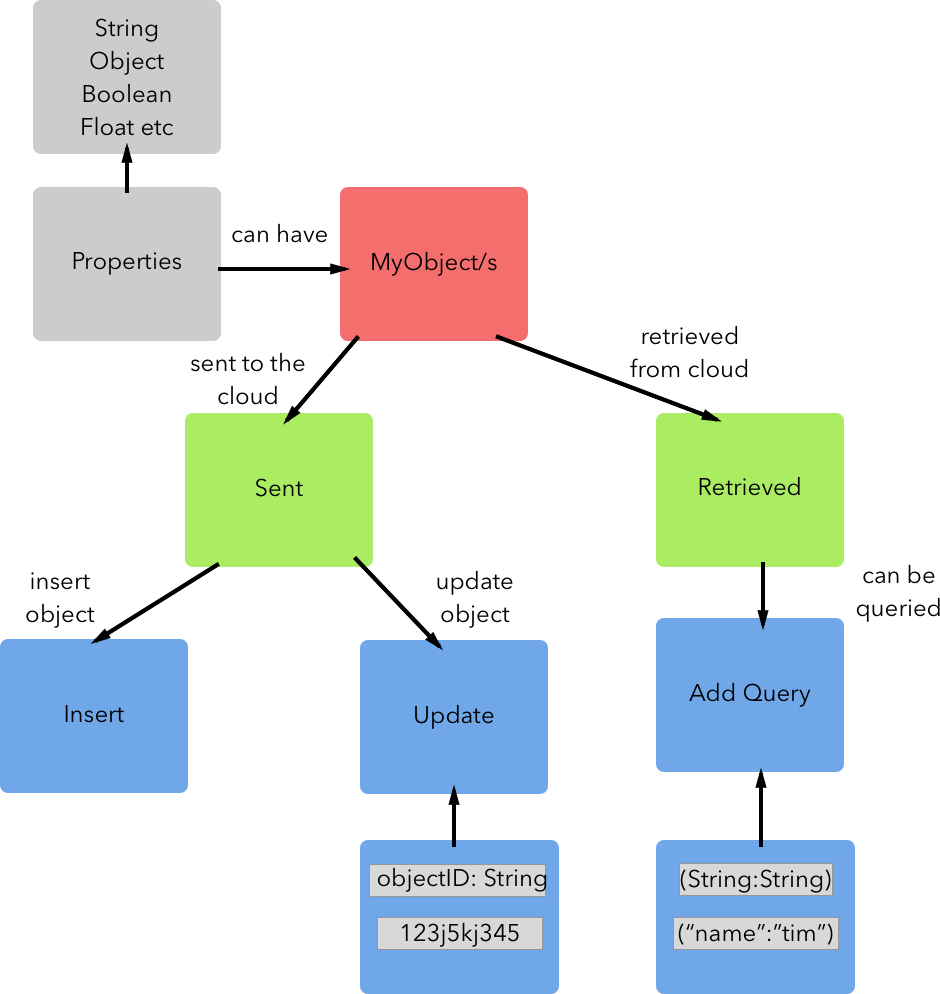
\includegraphics[width=100mm]{images/design/objects}
    \label{fig:sdk_storage}
\end{figure}

Figure \ref{fig:sdk_storage} illustrates the design of the storage library. The objects that the developers require for their app will all need the same functionality, being the way that the objects exchange information with the server. This then states that they all need to conform to the same way, and this is done using a protocol. The storage library will contain an object-relational mapping (ORM) tool, that will speed up parsing the objects to and from JSON format. This way the developer does not need to understand JSON format, but that the functionality is there to handle it. The last part of the design is that the properties being sent to the server will always be of type \textit{String}. The reasoning for this, is that if the developer decides to change their mind regarding the client app object property, it will not ruin the already stored data. The \textit{String} type is the only one that can handle all over types such as \textit{Int} and \textit{Boolean}. The development chapter will go into detail what protocol in software terms mean and how it is implemented within the storage library. 

\subsubsection{APNs} \label{d-sdk:apns}

\begin{figure}[!h]
    \caption{Notification SDK Design}
    \centering
    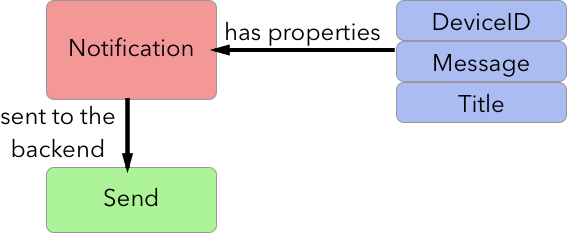
\includegraphics[width=100mm]{images/design/notification}
    \label{fig:apns_storage}
\end{figure}

Apple push notifications as stated above provides a way for apps to alert the user that an action has occurred. This action can be a text message or a friend that has been added. The notifications have to be activated by a sender, so when the user sends a message, a notification object will be sent to the server and in turn to the receiver. The library will contain a notification class, that will contain the required properties and the functionality to send the notification as illustrated in figure \ref{fig:apns_storage}.

\subsubsection{Analytics} \label{d-sdk:analytics}

\begin{figure}[!h]
    \caption{Notification SDK Design}
    \centering
    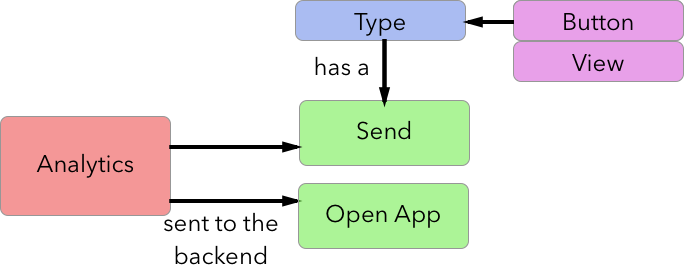
\includegraphics[width=100mm]{images/design/analytics}
    \label{fig:analytics_design}
\end{figure}

The analytics library as illustrated in figure \ref{fig:analytics_design}, has the capabilities of sending categorised types of analytics to the server. The type can be when a user clicks a button, or when a view is opened. The class will contain many different functionalities to make it easier for the developer to use. An example can be seen in \ref{fig:analytics_design} where the open app function is straight forward to send.

\subsubsection{Remote Configuration/Language} \label{d-sdk:rc_l}

\begin{figure}[!h]
    \caption{RC/Language SDK Design}
    \centering
    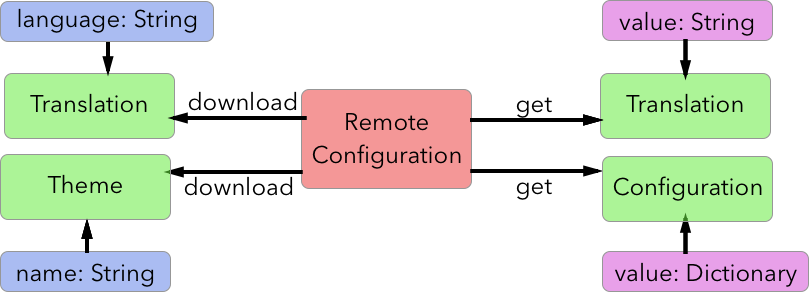
\includegraphics[width=120mm]{images/design/remote_config}
    \label{fig:remote_config_design}
\end{figure}


\begin{figure}[!h]
    \caption{RC File Design}
    \centering
    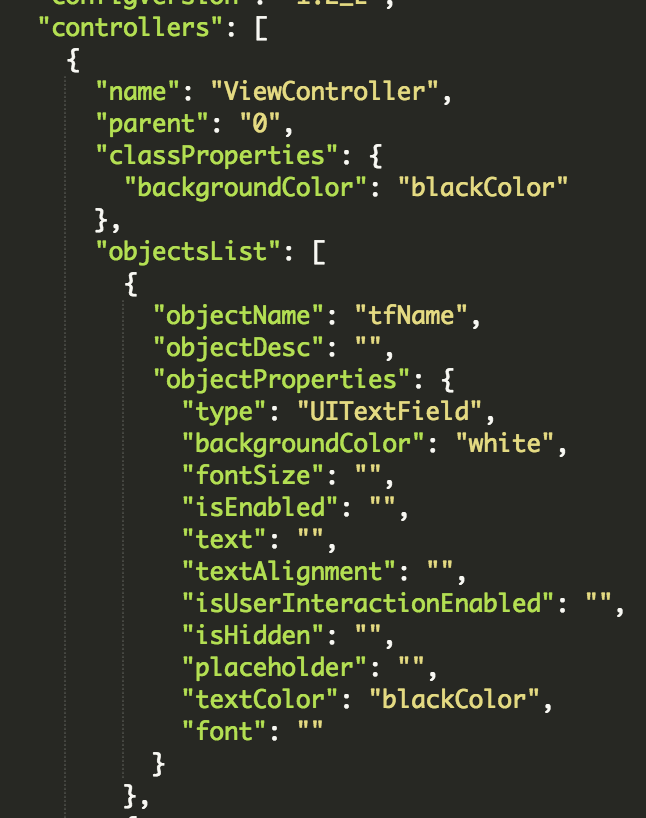
\includegraphics[width=70mm]{images/design/rc_file}
    \label{fig:rc_file_design}
\end{figure}

This section contains two parts: remote configuration and language. The are designed together as they both use the same system to update the application remotely. Figure \ref{fig:remote_config_design} shows two components of the library, where one part is for downloading the correct language and configuration file, the other to retrieve from. The downloading section for both takes a key parameter which distinguishes it from the other such as language name, or theme name, i.e., Dark, Light.  

The remote configurations and translations will be stored in JSON files, that can be both easily retrieved and stored on the device. Using the JSON files will speed up reading for each object properties. The structure of the configuration file as illustrated in \ref{fig:rc_file_design} contains an object inside a controller class, and then the properties of the object.

\subsection{Dashboard}

\subsubsection{Settings} \label{d-db:settings}

\begin{figure}[!h]
    \caption{Settings Use Case Diagram}
    \centering
    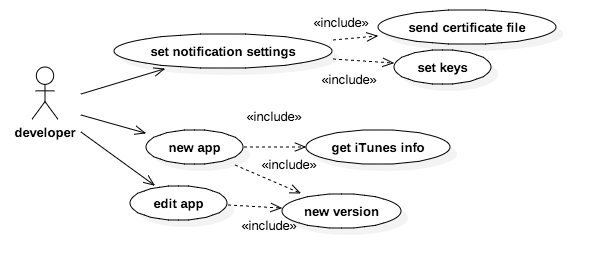
\includegraphics[width=100mm]{images/use_cases/settings_uc}
    \label{fig:settings_uc}
\end{figure}

The use case diagram for the settings views shown in \ref{fig:settings_uc}. The developer in this view can set up the notifications requirements such as sending the certificate file. This certificate is crucial for sending notifications; it authenticates the developer's id when about to send the notification object.

The next part of the settings view, the developer can create and edit applications. These apps are the mobile apps that will be used in conjunction with the web-server and the SDK. These apps and versions will be used throughout the rest of the dashboard when setting remote configuration for example. When an application is being updated, some key values can also be retrieved from the iTunes API.

\subsubsection{Storage} \label{d-db:storage}

Figure \ref{fig:storage_use_case} illustrates the storage/database use case. In the storage view in the dashboard, the developer will be able to choose a database which is specific to each application. After which be able to view and select the collections within and see the content records. Another feature is the ability to import collection from a JSON or CSV file into the database.

This use case is limited by design, the typical create, read, update and delete (CRUD) operations known with database development will not be available. When designing systems that include both backend and frontend, the most important one of two is the frontend. This is what the end users will see, so this system will focus on designing the structure of each collection in the application, in the development stage. 

Typically the dashboard will allow the developer to perform CRUD operations, and then they will have to mimic that structure for the frontend app, thereby creating a potential bug. A bug can occur if someone can change the collection name, or collection property name, thus creating an inconsistency between frontend and backend. Removing the capabilities from one side being backend will hopefully eliminate this potential issue.

\begin{figure}[!h]
    \caption{Storage View Use Case Diagram}
    \centering
    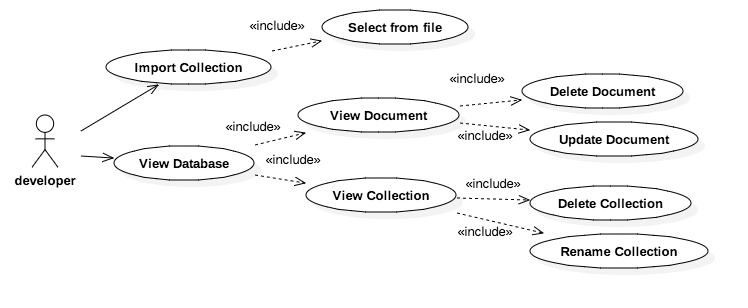
\includegraphics[width=120mm]{images/use_cases/storage_use_case}
    \label{fig:storage_use_case}
\end{figure}

\subsubsection{Notifications} \label{d-db:notifications}

\begin{figure}[!h] 
    \caption{APNs View Use Case Diagram}
    \centering
    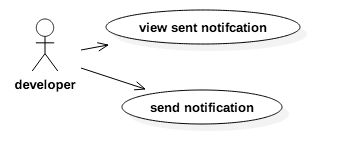
\includegraphics[width=80mm]{images/use_cases/notifications_uc}
    \label{fig:notifications_uc}
\end{figure}

Apple push notifications (APNs) that have sent can be viewed in the notifications view as illustrated in \ref{fig:notifications_uc}. The developer can also send notifications from the dashboard to the mobile apps, for example telling users about an update, or new theme, etc. 

\subsubsection{Remote Configuration} \label{d-db:remote_config}

\begin{figure}[!h]
    \caption{RC View Use Case Diagram}
    \centering
    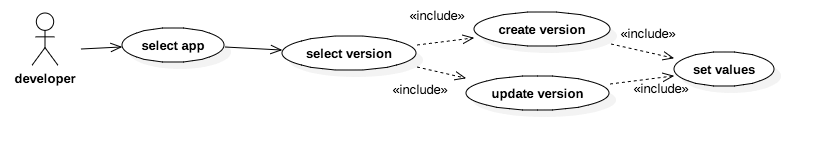
\includegraphics[width=100mm]{images/use_cases/rc_uc}
    \label{fig:rc_uc}
\end{figure}
 
The developer in the remote configuration view once an application and version have been chosen can create versions. These versions define the user interface of the mobile app. Each version will be dependent on an app version or a particular theme. In figure \ref{fig:rc_uc} illustrates what the capabilities of this view. After a version is created or being updated, the properties for the UI objects such as a label can be set.
 
\subsubsection{Languages} \label{d-db:languages}

\begin{figure}[!h]
    \caption{Language View Use Case Diagram}
    \centering
    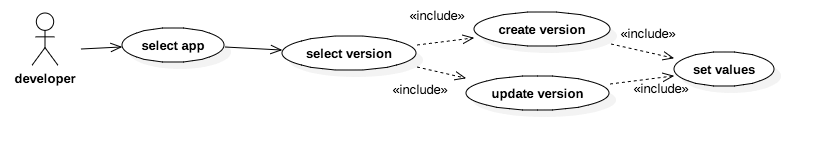
\includegraphics[width=100mm]{images/use_cases/rc_uc}
    \label{fig:language_uc}
\end{figure}

The language view use case in figure \ref{fig:language_uc} is similar to the remote configuration use case above. This is because both are designed in the same way, that each version can be downloaded and the data is retrieved in the app.

\subsubsection{Backup} \label{d-db:backup}

\begin{figure}[!h]
    \caption{Backup View Use Case Diagram}
    \centering
    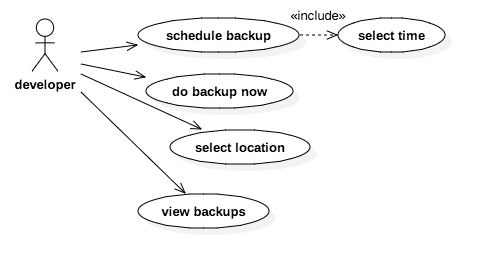
\includegraphics[width=80mm]{images/use_cases/backup_uc}
    \label{fig:backup_uc}
\end{figure}

The backup view is where the developer can either set up a scheduled backup or do a backup now. In the use case figure \ref{fig:backup_uc}, all the previous backups can be seen in this view. The developer will also be able to select a location for these backups placed, being either remotely or locally. The backups will have the time-stamp and zipped to help save space.

\subsection{Web Server} \label{d-web_server}

\begin{figure}[!h]
    \caption{Web Server Design}
    \centering
    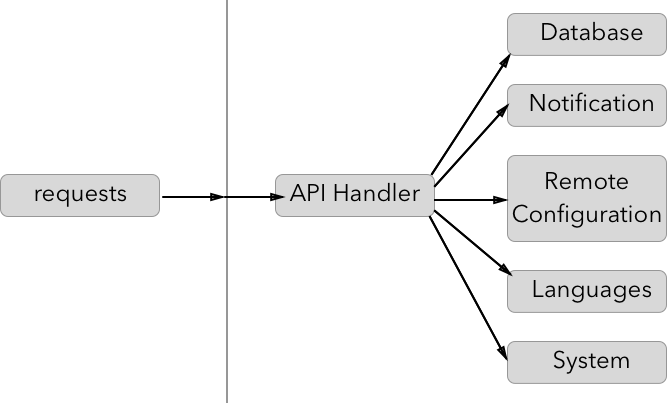
\includegraphics[width=100mm]{images/design/api_handler}
    \label{fig:api_handler}
\end{figure}

The web server brief design is illustrated in \ref{fig:api_handler}. The web server uses an application programming interface (API) which defines a set of methods for communication. In this system, the database and notifications are an example of defined tools that will be used. The API Handler takes the request in and forwards it on to the correct web app to handle the request, and relay a response back. The development chapter under web server section will discuss in detail the list of tools.


\section{Design Principles}

Human-Computer Interaction (HCI) principles play a major role when designing an interface. These principles help keep applications of the same nature alike. An example is a mail app, the icon for a mailbox or sending messages can be used to convey without having to read a manual of what a button does. As this system will be using a Mac application, the macOS interface guidelines will be closely followed.

Apples Human Interface Guidelines \cite{guidelines} discussed the following design principles:

\begin{enumerate}
  \item Mental Model 
  
  - "..is the concept of an object or experience that people carry in their heads". It is the model of what users believes about the system, so the mental model of past experience on similar systems will be carried when looking to use this system. This will involve looking at current systems available and design the interface somewhat similar.
  
  \item Direct Manipulation
  
  - ”..is an example of an implied action that helps users feel that they are controlling the objects represented by the computer”. When designing a view that the user can control, the objects such as deleting a record should only become invisible once the user has taken action.
  
  \item User Control 
  
  - ”..principle of user control presumes that the user, not the computer, should initiate and control actions.” The interface should give the user the control depending on the type of user. So a professional user will want more power compared to a novice user.
  
  \item Consistency
  
  - "..allows the user to transfer their knowledge and skills from one app to another". So by designing the system will the same general layout of other apps will help the user not feel lost.
  
\end{enumerate}